\documentclass[12pt, a4paper, openany]{book}
\usepackage[inline]{enumitem}
\usepackage{../generalStyle}
\usepackage{graphicx}
\usepackage{float}
\usepackage{amsmath}


\begin{document}

\title{Formulario di Fisica}
\author{Gianluca Parpanesi}
\date{2022/2023}
\maketitle

\tableofcontents
\newpage

\section*{Nozioni Generiche}

\begin{itemize}
    \item La velolcità di un corpo è identificata come lo spostamento sul tempo:
        \begin{equation*}
            v = \frac{dx}{dv}
        \end{equation*}
    \item L'accelerazione di un corpo è identificata come la velocità sul tempo:
        \begin{equation*}
            a = \frac{dv}{dt}
        \end{equation*}
    \item La massa non influisce sul tempo di caduta dovuto da un campo 
        gravitazionale. Due oggetti con masse completamente diverse subiscono la
        stessa identica accelerazione.
    \item Una forza è conservativa se il Lavoro netto che una particella compie
    in un percoso chiuso è 0. In modo equivalente, una forza è conservativa 
    se il Lavoro netto che compie una particella in movimento non dipende dal 
    percorso che essa compie. La forza gravitazionale e la forza elastica sono
    forze conservative, l'attrito dinamico non è una forza conservativa.
    
    \paragraph{Prodotto tra vettori} Il prodotto tra due vettori può essere 
    eseguito in due modi differenti: il primo tipo di prodotto dà origine ad uno
    scalare (prodotto scalare) mente l'altro darà origine ad un vettore 
    (prodotto vettoriale).
    \begin{itemize}
        \item \textbf{Prodotto scalare}: il prodotto scalare dei vettori $a$ e
        $b$ si scrive $a \cdot b$ ed è definito dall'espressione
        \begin{equation*}
            a \cdot b = ab \cos \Theta
        \end{equation*}
        dove $a$ è il modulo del vettore $\boldsymbol{a}$, $b$ il modulo del 
        vettore $\boldsymbol{b}$ e $\Theta$ è l'angolo formato dalle semirette 
        equiverse su cui giacciono i due vettori.
        \item \textbf{Prodotto vettoriale}: il prodotto vettoriale 
        dei vettori $a$ e $b$ si scrive $a \times b$ ed è definito 
        dall'espressione
        \begin{equation*}
            a \times b = ab \sin \Theta
        \end{equation*}
        dove $a$ è il modulo del vettore $\boldsymbol{a}$, $b$ il modulo del 
        vettore $\boldsymbol{b}$ e $\Theta$ è il minore dei due angoli formati 
        dalle semirette equiverse su cui giacciono i due vettori. 
        La direzione del vettore risultante è \textbf{perpendicolare} al piano 
        individuato da $a$ e $b$.
    \end{itemize}
    
\end{itemize}

\chapter{Cinematica}

    \section{Moto rettilineo uniforme}

        \paragraph{Velocità} 
            La velocità viene rappresentata da uno scalare:
            \begin{equation}
                v_x = k
            \end{equation}

        \paragraph{Velocità media} 
            La velocità media viene rappresentata come un intervallo di uno 
            spostamento su un intervallo di tempo:
            \begin{equation}
                v_m = \frac{\Delta x}{\Delta t} = \frac{x_f - x_i}{t_f - t_i}
            \end{equation}

        \paragraph{Velocità istantanea} detta anche semplicemente velocità di 
        una particella, è definita come:
            \begin{equation}
                v = \lim_{x \to 0}  \frac{\Delta x}{\Delta t} = \frac{dx}{dt}
            \end{equation}

        \paragraph{Spostamento}
            \begin{equation}
                x(t) = x_i + v_xt
            \end{equation}

    \section{Moto uniformemente accelerato}

        \paragraph{Accelerazione media} è il rapporto fra la variazione della
        velocità $\Delta v$ che avviene in un intervallo di tempo $\Delta t$, 
        definita come:
        \begin{equation}
            a_m = \frac{\Delta v}{\Delta t} = \frac{v_f - v_i}{t_f - t_i}
        \end{equation}

        \paragraph{Accelerazione istantanea} o semplicemente accelerazione, è 
        la rapidità di variazione della velocità. Matematicamente si tratta 
        della derivata seconda della posizione $x(t)$ rispetto al tempo:
        \begin{equation}
            a = \frac{dv}{dt} = \frac{d^2x}{dt^2}
        \end{equation}

        \paragraph{Spostamento}
            \begin{equation}
                x(t) = x_i + v_it + \frac{1}{2}at^2
            \end{equation}

        \paragraph{Velocità finale}
            \begin{equation}
                v_f(t) = v_{i} + at
            \end{equation}
    
        \paragraph{Caso particolare}
            Per determinare il tempo possiamo effettuare la fomrula inversa 
            dello spostamento. È possivile notare come il tempo non dipende 
            dalla massa degli oggetti, ma dall'altezza e dalla forza di gravità
            . In assenza d'aria di conseguenza due oggetti con masse 
            completamente diverse arrivano a terra allo stesso tempo!

            \begin{equation}
                t_c=\sqrt{\frac{2h}{g}}
            \end{equation}

    \section{Moto di un proiettile} 

        Il moto di un proiettile è scomponibi le lungo gli assi cartesiani in 
        due moti ben distinti, agenti su un unico corpo:
        \begin{itemize}
            \item \textbf{Asse X}: moto rettilineo uniforme.
            \item \textbf{Asse Y}: moto rettilineo uniformemente accelerato.
        \end{itemize}
        Soffermandoci su questo ragionamento possiamo notare come la forza di 
        gravità (accelerazione) agisca in modo costante lungo l'asse y 
        effettuando un'accelerazione negativa (decelerazione) lungo questa 
        componente del moto. Il moto dell'asse x invece non viene intaccato da 
        nessun'altra forza (trascurando ovviamente l'attrito dell'aria).
        
        \paragraph{Equazioni del moto}
        (Per assi cartesiani)
        \begin{align}
            x &: x(t) = x_0 + v_{0x}t \\
            y &: \begin{cases}
                    y(t) &= y_0 + v_{0y}t + \frac{1}{2}at^2 \\
                    v_{fy} &= v_{0y} + at
                \end{cases}
        \end{align}

    \section{Moto circolare uniforme}
        Nel moto circolare uniforme agiscono 3 forze:
        \begin{itemize}
            \item Velocità tangenziale
            \item Accelerazione centripeta
            \item Accelerazione centrifuga
        \end{itemize}
        Le prime due sono forze fisiche reali, mentre la terza è chiamata forza
        apparente. Difatti la forza che ci fa sentire spinti verso l'esterno è
        data dalla nostra inerzia nel tendere a proseguire il nostro moto 
        diritti, mentre l'accelerazione centripeta (sempre rivolta verso il
        centro della curva) ci tiene in traiettoria circolare. Questo accade
        perché ci troviamo in un sistema non inerziale: difatto se lanciassimo 
        una pallina mentre ci troviamo all'interno di un moto circolare essa ci
        sembrerà allontanarsi da noi con una sua traiettoria, spinta da una 
        forza (apparente) verso l'esterno. Vista da un osservatore posto al di
        fuori del moto (in un sistema inerziale) semplicemente la pallina 
        proseguirà diritta nella sua traiettoria.\\\\
        Analizziamo ora le formule del moto circolare uniforme:

        \paragraph{Velocità tangenziale} La velocità tangenziale è lo spazio 
        percorso dal punto materiale in un intervallo di tempo:
        \begin{equation}
            v = \frac{2\pi r}{T}
        \end{equation}

        \paragraph{Accelerazione centripeta} L'accelerazione centripeta è 
        quella forza che mantiene un corpo in un moto circolare uniforme. Essa
        è sempre diretta verso il centro della circonferenza!.
        \begin{equation}
            a_c = \frac{v^2}{r}=
        \end{equation}
        Come vedremo più avanti in questo formulario l'accelerazione è impressa
        da una forza agente sul corpo, descrivibile (tramite la Seconda Legge
        di Newton) come:
        \begin{equation}
            F_{accelerazione} = ma = m\frac{v^2}{r}
        \end{equation}

        \paragraph{Periodo} Il tempo richiesto perché una particella completi
        una circonferenza è:
        \begin{equation}
            T = \frac{2\pi r}{v}
        \end{equation}

    
        \subsection{Moto Armonico}  \label{moto_armonico}
        Il moto circolare uniforme può essere scomposto in due moti sinusoidali 
        $\sin$ e $\cos$.
        Il moto circolare uniforme e quello uniformemente accelerato possono 
        essere perfettamente paragonati al moto rettilineo uniforme e quello 
        uniformemente accelerato. In questo caso $\Theta$ è la nostra $x$ 
        mentre la velocità $v$ diventa $\omega$.\\\\
        Nel caso uniformemente accelerato l'accelerazione $a$ diventa $\alpha$.

        \paragraph{Legge oraria (equazione del moto)} Essa descrive il moto del
        moto circolare uniforme, espresso come angolo in funzione del tempo:
        \begin{equation}
            \Theta = \Theta_0 + \omega t = 
            \begin{cases}
                x(t)=R\cos{\Theta(t)} \\
                y(t)=R\sin{\Theta(t)}
            \end{cases} 
            = 
            \begin{cases}
                x(t)=R\cos{(\Theta_o+\omega t)} \\
                y(t)=R\sin{(\Theta_o+\omega t)}
            \end{cases}
        \end{equation}

        \paragraph{Velocità angolare} La velocità angolare è l'angolo percorso
        dal punto materiale in un intervallo di tempo:
        \begin{equation}
            \omega = \frac{2\pi}{T}
        \end{equation}
        Espressa in radianti al secondo.

        \paragraph{Velocità tangenziale} La velocità tangenziale è lo spazio 
        percorso dal punto materiale in un intervallo di tempo:
        \begin{equation}
            v = \frac{2\pi r}{T} = 
            \begin{cases}
                v_x=-R\omega\sin{(\Theta_o+\omega t)} \\
                v_y=R\omega\cos{(\Theta_o+\omega t)}
            \end{cases}
        \end{equation}

        \begin{quote}
            Da notare come (per definizione) le equazioni della velocità non 
            sono altro che la derivata ' dell'equazione del moto 
            (Legge oraria)! 
        \end{quote}

        \paragraph{Accelerazione centripeta} L'accelerazione centripeta è 
        quella forza che mantiene un corpo in un moto circolare uniforme. Essa
        è sempre diretta verso il centro della circonferenza!.
        \begin{equation}
            a_c = \frac{v^2}{r}=
            \begin{cases}
                a_x=-R\omega^2\cos{(\Theta_o+\omega t)} \\
                a_Y=-R\omega^2\sin{(\Theta_o+\omega t)}\end{cases}
        \end{equation}

        \begin{quote}
            Da notare come (per definizione) le equazioni dell'accelerazione 
            non sono altro che la derivata " dell'equazione del moto 
            (Legge oraria)! 
        \end{quote}
        
    \section{Moto circolare uniformemente accelerato} Nel moto circolare 
    uniformemente accelerato entra in gioco l'accelerazione totale come somma
    vettoriale dell'accelerazione centripeta e dell'accelerazione tangeziale.
    Di conseguenza l'equazione del moto sarà il sistema:

        \paragraph{Legge oraria (equazione del moto)}
        \begin{equation}
            \begin{cases} 
                \Theta = \Theta_0 + \omega_0t + \frac{1}{2}\alpha t^2 \\ 
                \omega = \omega_0+\alpha t
            \end{cases}
        \end{equation}

        \subsection{Tabelle di riepilogo} Di seguito sono riportate due tabelle 
        contententi un riepilogo delle formule (comprese le formule inverse) 
        sia del Moto circolare uniforme \ref{fig:MCU} che del Moto circolare 
        uniformemente accelerato \ref{fig:MCUA}.

        \begin{figure}[H]
            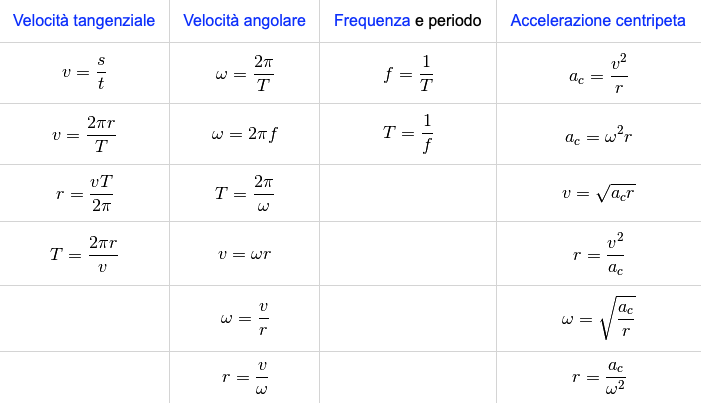
\includegraphics[width=0.9\linewidth]
            {formulario/img/Formulario_MCU.png}
            \caption{Formule del Moto circolare uniforme}
            \label{fig:MCU}
        \end{figure}

        \begin{figure}[H]
            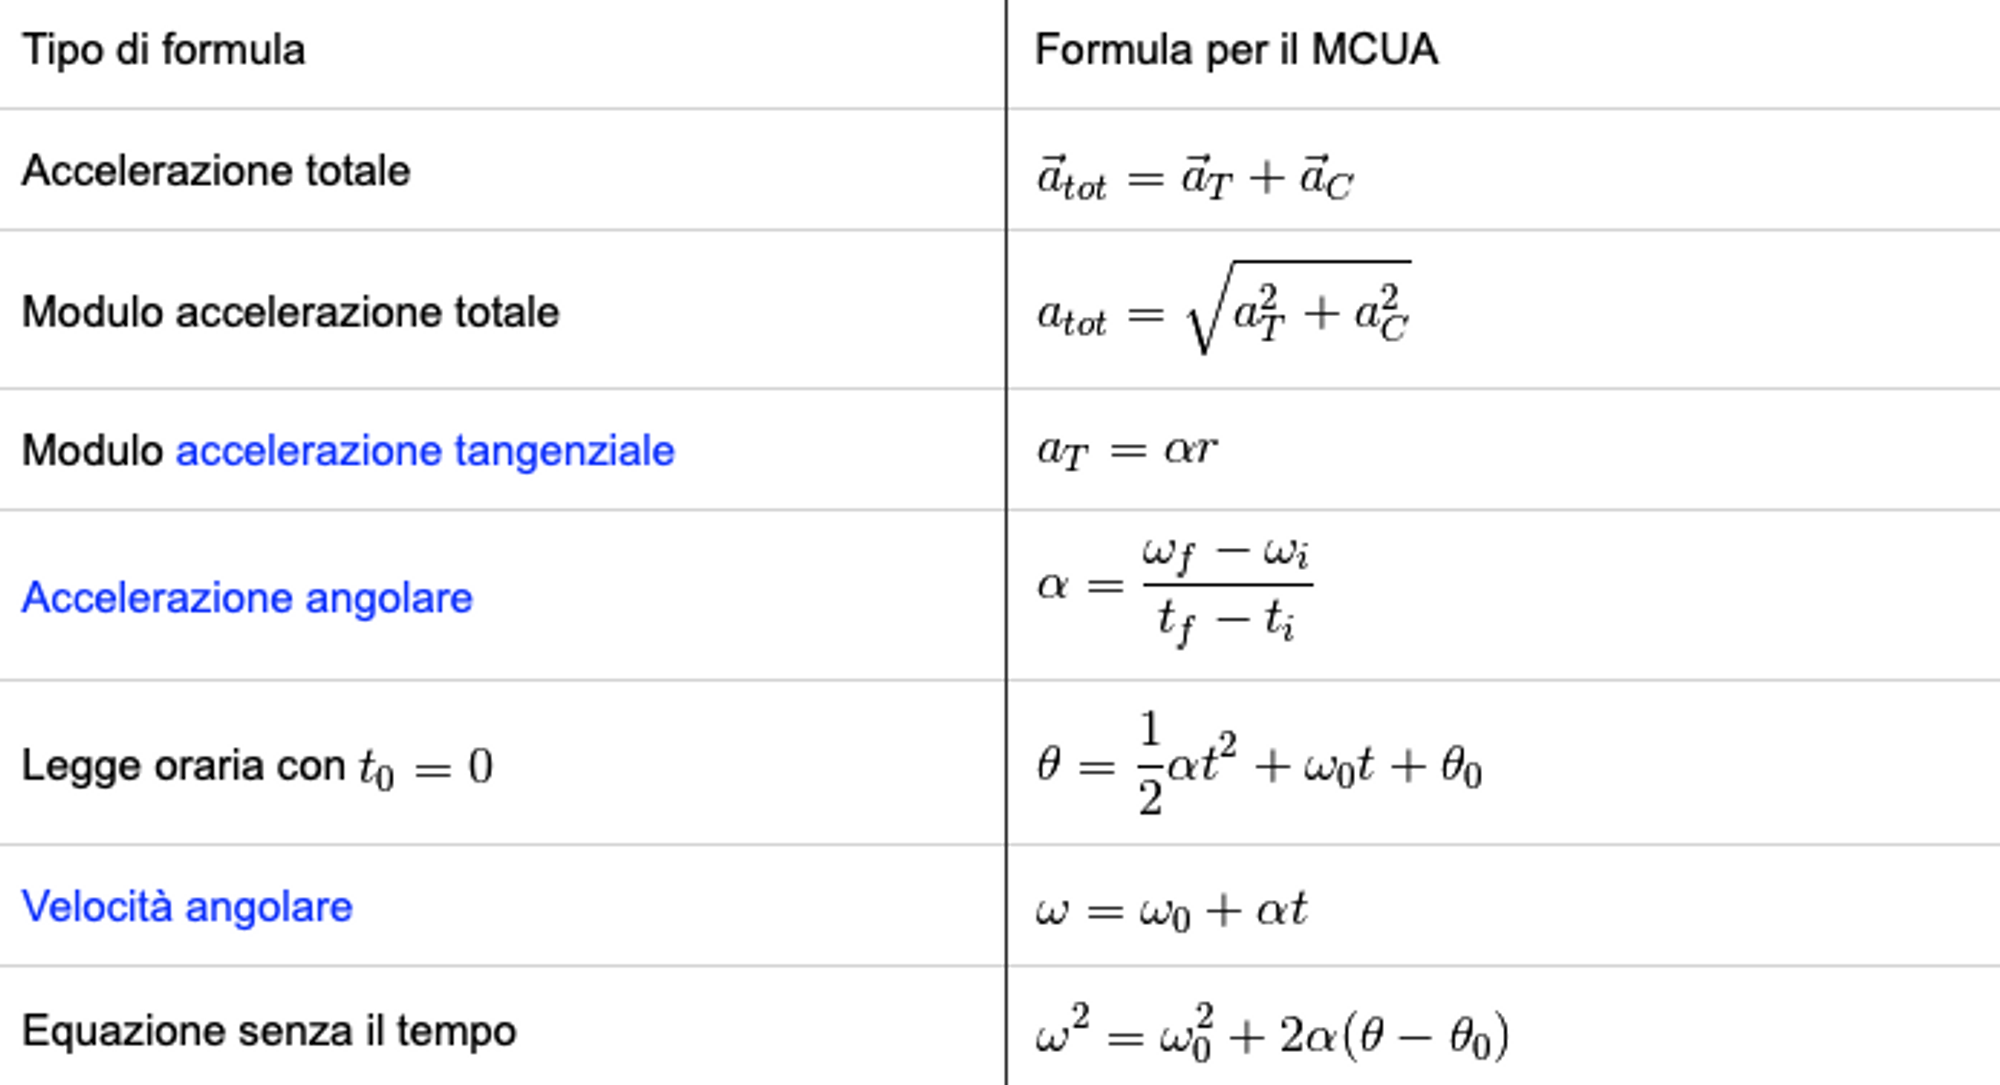
\includegraphics[width=0.9\linewidth]
            {formulario/img/Formulario_MCUA.png}
            \caption{Formule del Moto circolare uniformemente accelerato}
            \label{fig:MCUA}
        \end{figure}

        

\chapter{Dinamica}

    \section{Principi della Dinamica - Leggi di Newton}

        \paragraph{Prima Legge di Newton} Se la somma delle forze che agiscono 
        su un corpo è nulla, allora il corpo in quiete rimarrà in quiete, mentre
        se è in moto, continuerà a muoversi di moto rettilineo uniforme.

        \paragraph{Seconda Legge di Newton} La forza agente su un corpo è 
        direttamente proporzionale all'accelerazione e ne condivide la direzione
        e il verso, ed è direttamente proporzionale alla massa. Di contro 
        l'accelerazione cui è soggetto il corpo è direttamente proporzionale 
        alla forza e inversamente proporzionale rispetto alla massa.

        \begin{equation}
            \vec{F} = m \vec{a} \; [N]
        \end{equation}

        \paragraph{Terza Legge di Newton} Se un corpo A esercita una forza su 
        un corpo B, allora il corpo B esercita su A una forza uguale e 
        contraria.

        \begin{equation}
            F_{ab} = - F_{ba}
        \end{equation}

        \begin{quote}
            Attenzione! Le forze hanno modulo uguale ma con segno vettoriale 
            opposto!
        \end{quote}

    \section{Forza Elastica} La forza elastica di un corpo (o di una molla) è 
    descritta dalla Legge di Hook nel seguente modo:
        \begin{equation}
            F = -kx
        \end{equation}
    Dove $-k$ è chiamata \textbf{costante elastica} ed è una misura della 
    rigidità della molla. Maggiore è $k$, più rigida è la molla: cioè maggiore è
    $k$, maggiore sarà la forza per uno stesso valore di spostamento.

    \section{Carrucola} Le forze agenti su due corpi collegati in un sistemma a
    carrucola (se aventi masse diverse) sono sempre una l'opposta dell'altra.
        \begin{equation}
            \begin{cases}
                F_{y1} = T - m_1g \\
                F_{y2} = m_2g - T
            \end{cases}
        \end{equation}
    In questo caso si considera $m_2 > m_1$ e con un sistema di riferimento 
    verticale. Si considera infatti un sistema a carrucola con forze agenti solo
    sull'asse $y$ e con forze nulle sull'asse $x$.

    \section{Attrito Statico e Dinamico} La forza di attrito è una forza che 
    agisce in direzione opposta allo spostamento (opponendosi al movimento). La 
    forza di attrito può agire in due modi differenti:
        \begin{itemize}
            \item \textbf{Attrito statico}: agente quando il corpo è fermo, 
            impedendo lo spostamento iniziale.
            \item \textbf{Attrito dinamico}: agente da quando il corpo ha appena 
            compiuto lo spostamento iniziale ed è in movimento.
        \end{itemize}
    Le formule sono per l'attrito statico:
        \begin{equation}
            f_{s, max} = \mu_sF_N
        \end{equation}
        Mentre per quello dinamico:
        \begin{equation}
            f_{k} = \mu_kF_N
        \end{equation}
    
    \section{Resistenza di un corpo} Quando un corpo solido si muove 
    all'interno di un fludio, ad esso si oppone una forza contraria chiamata
    resistenza $D$ la quale farà raggiungere al corpo una velocità massima:
        \begin{equation}
            D = \frac{1}{2}CA\rho v^2
        \end{equation}
        Con:
        \begin{itemize}
            \item C : Coefficiente di resistenza aerodinamica.
            \item A : Area efficace della sezione trasversale del corpo.
            \item $\rho$ : densità dell'aria
            \item v : velocità.
        \end{itemize}

    \section{Lavoro} Si applichi una forza F ad un oggetto per spostarlo. La 
    Forza sarà tanto efficace ad ottenere uno spostamento \textbf{tanto più
    è applicata nella stessa direzione dello spostamento.}

        \begin{equation}
            W = Fd = Fd \cos \Theta \; [J]
        \end{equation}

        \paragraph{Lavoro compiuto dalla Forza Gravitazionale} Il Lavoro svolto 
        dalla Forza Gravitazionale ovviamente è descritto come $F d$, per un 
        corpo che sale la $F_g$ è diretta in senso opposto allo spostamento 
        formando un angolo $\Theta$ di $180^{\circ}$.
        
        \begin{equation}
            F = mgd\cos \Theta = mgd \cos 180 = - mgd
        \end{equation}
        Mentre nel momento in cui un corpo cade, la $F_g$ avrà stessa direzione
        dello spostamento (verso il basso), conferendo un segno positivo al
        Lavoro.
        
        \paragraph{Lavoro compiuto dalla Forza Elastica} La Forza Elastica non è
        una forza costante e di conseguenza non possiamo utilizzare la classica
        equazione del Lavoro (per una forza costante). Possiamo però suddividere
        lo spostamento della molla in parti infinitesime in modo da avere forze
        infinitesime per ogni spostamento infinitesimo, facendo risultare cosi 
        la forza infinitesima costante su uno spostamento infinitesimo. 
        Integrando questa operazione otterremo così la formula del lavoro per
        la Forza Elastica (e in generale per una forza non costante!).
        \begin{equation*}
            L_m = \int_{x_f}^{x_i} -F \,dx 
        \end{equation*}
        \begin{equation*}
            L = \int_{x_f}^{x_i} -kx \,dx =  L = -k \int_{x_f}^{x_i} x \,dx   
        \end{equation*}
        \begin{equation*}
            = (-\frac{1}{2}k)\bigg[x^2 \bigg]_{x_f}^{x_i}
            = (-\frac{1}{2}k) (x^2_f - x^2_i)
        \end{equation*}
        \begin{equation}
            L_m = \frac{1}{2}kx^2_i - \frac{1}{2}kx^2_f
        \end{equation}
        Il Lavoro $L_m$ è positivo quando il blocco si avvicina alla posizione 
        di riposo $x=0$ ed è negativo quando se ne allontana. Il Lavoro è nullo
        se la distanza finale da $x=0$ non è mutata.

    \section{Energia Cinetica} Rappresenta la quantità di energia associata al 
        moto di una particella (corpo puntiforme) che si muove alla velocità $v$.

        \begin{equation}
            K = \frac{1}{2}mv^2 \; [J]
        \end{equation}

        \begin{quote}
            Il lavoro fatto su una particella è uguale a $\Delta K$. L'energia 
            cinetica (e la velocità) aumentano se il lavoro svolto è positivo, 
            mentre diminuiscono se il lavoro svolto è negativo.
        \end{quote}

        \paragraph{Teorema dell'Energia Cinetica} Chiamiamo $\Delta K$ la 
        variazione di Energia Cinetica del corpo e $L$ il Lavoro totale compiuto
        su di esso. Allora possiamo scrivere:
        \begin{equation}
            \Delta K = K_f - K_i = W
        \end{equation}

        \paragraph{Energia Cinetica del Moto Armonico Semplice} Si consideri un
        sistema molla-blocco, nel caso senza attriti, possiamo visualizzare il 
        suo andamento come un'oscillazione armonica e descrivere la sua Energia
        Cinetica come:
        \begin{equation}
            K = \frac{1}{2}mv^2 = \frac{1}{2}m\omega^2A^2\sin^2
            (\Theta + \omega t)
        \end{equation}

    
    \section{Potenza} Se una forza esterna è applicata ad un oggetto e se il 
    Lavoro è fatto in un intervallo di tempo, definiamo \textbf{potenza}:
        
        \begin{equation}
            P = \frac{W}{\Delta t} \; [W \textsf{  Watt}]
        \end{equation}

        \paragraph{Un altro sguardo alla Potenza} La Potenza Istantanea può 
        essere espressa derivando la formula della Potenza (ovviamente!). Di 
        conseguenza possiamo scrivere la potenza come:

        \begin{equation*}
            P = \frac{dL}{dt} = \frac{F \cos \Theta dx}{dv} 
            = F \cos \Theta (\frac{dx}{dt})
        \end{equation*}
        Ma sappiamo benissimo che $\frac{dx}{dv}$ non è altro che la definzione 
        di velocità. Possiamo quindi riscriverla in modo più semplice:
        \begin{equation*}
            P = Fv\cos\Theta
        \end{equation*}
        Ovvero il \textbf{prodotto scalare} tra $F$ e $v$ (dove $v$ è la 
        velocità della particella). Possiamo quindi scrivere che la Potenza 
        Istantanea di una paricella a velocità $v$ non è altro che:
        \begin{equation}
            P = F \cdot v
        \end{equation}

    \section{Energia Potenziale} Se la configurazione di un sistema cambia, 
    allora cambierà anche la sua Energia potenziale. Quando un oggetto si trova
    ad una certa distanza dal suolo, il sistema terra-oggetto ha un'energia 
    potenziale che si trasforma in lavoro. \\
    L'Energia Potenziale è associata con la configurazione del sistema nel quale
    le forze conservative agiscono. Quando una forza conservativa compie lavoro
    $W$ su una particella (corpo) del sistema, il cambiamento $\Delta U$ 
    dell'energia potenziale del sistema è definito come:
        
        \begin{equation}
            \Delta U = - W
        \end{equation}

        \paragraph{Energia Potenziale Gravitazionale} L'energia potenziale in un
        sistema composto dalla terra e dalla particella (corpo) è chiamata 
        Energia Potenziale Gravitazionale. Se la particella si muove da 
        un'altezza iniziale $y_i$ ad una finale $y_f$, il cambiamento 
        dell'Energia Potenziale Gravitazionale è definito come:
        \begin{equation}
            \Delta U = mg(y_f - y_i) = mg \Delta y
        \end{equation}
        Se considerassimo come punto di arrivo un altezza $= 0$, allora 
        l'Energia Potenziale gravitazionale piò essere riscritta come:
        \begin{equation}
            \Delta U(h) = mgh
        \end{equation}
        Dove $h$ è l'altezza dalla quale il corpo cade.

        \paragraph{Energia Potenziale Elastica} L'energia Potenziale Elastica è 
        l'energia associata allo stato di compressione o estensione di un 
        oggetto elastico (molla). Per una molla con una forza definita come 
        $ F = -kx $, l'Energia Potenziale Elastica sarà definita come:
        \begin{equation}
            U(x)     = \frac{1}{2}kx^2
        \end{equation}

        \paragraph{Energia Potenziale del Moto Armonico Semplice} L'energia 
        Potenziale Elastica di un oscillatore armonico, immagazzinata dalla 
        molla a seguito di un allungamento $x$ è:
        \begin{equation}
            U = \frac{1}{2}kx^2 = \frac{1}{2}kA^2\cos^2(\Theta + \omega t)
        \end{equation}

    \section{Energia Meccanica} La somma dell'Energia Cinetica e dell'Energia
    Potenziale è detta Energia Meccanica, definita come:

        \begin{equation}
            E_m = K + U
        \end{equation}

        \paragraph{Principio di conservazione dell'Energia Meccanica} Quando in 
        un sistema isolato agiscono solo forze conservative, l'Energia Cinetica 
        e l'Energia Potenziale prese singolarmente possono variare, ma la loro
        somma, l'Energia Meccanica $E_m$ del sistema non cambia. Questo 
        risultato è chiamato principio di conservazione dell'Energia Meccanica
        espirmibile nel seguente modo:
        \begin{equation}
            \Delta E_m = \Delta K + \Delta U = 0
        \end{equation}
        Il principio di conservazione dell'Energia Meccanica ci permette di 
        risolvere problemi che sarebbe arduo risolvere usando solo le Leggi di 
        Newton.
        Quando l'Energia Meccanica di un sistema si conserva, possiamo mettere
        in relazione il totale dell'Energia Cinetica e dell'Energia Potenziale
        in un istante con quello di un altro istante, \textit{senza dover
        considerare gli stati intermedi e senza necessità di conoscere il lavoro
        compiuto dalle forze coinvolte!}

        \paragraph{Principio esteso} La variazione dell'Energia Meccanica è 
        uguale al lavoro svolto dalle Forze non conservative:
        \begin{equation}
            \Delta E_m = W_{nc}
        \end{equation}
        

    \section{Moto Armonico e Pendolo} L'oscillatore armonico può essere 
    rappresentato da un sistema molla-blocco il quale oscillando descrive un 
    moto circolare uniforme. Le equazioni del moto sono le stesse del Moto 
    Circolare Uniforme \ref{par_mcu},
        \begin{equation}
            x(t) = A \cos(\Theta_0 + \omega t)
        \end{equation}
        ma con:
        \begin{equation*}
            \omega = \sqrt[]{\frac{k}{m}}
        \end{equation*}
        ricordando l'equazione dei un sistema molla-blocco:
        \begin{equation*}
            F = -kx
        \end{equation*}
        
        \paragraph{Il pendolo} Il pendolo può essere descritto tramite il
        Moto Circolare Uniformemente Accelerato, considerando la lunghezza del 
        filo inestensibile come il raggio della circonferenza. In questo caso 
        abbiamo:
        \begin{equation*}
            \omega = \sqrt[]{\frac{g}{L}}
        \end{equation*}
    
    
    
    \section{Momento Lineare}

        \begin{equation}
            p = mv
        \end{equation}

        \paragraph{Connessione con la II Legge di Newton} Deriviamo il 
        Momento Lineare rispetto al tempo. La derivata della quantità di moto di
        un punto materiale di massa $m$ è uguale alla risultante della forza 
        applicata.

        \begin{equation*}
            \frac{dp}{dt} = \frac{d(mv)}{dt} = ma
        \end{equation*}

        \begin{equation*}
            \frac{dm}{dt} v + m \frac{dv}{dt} = ma
        \end{equation*}

        \begin{quote}
            Ma la massa rimane costante nel tempo, quindi la derivata sarà 0.
        \end{quote}

        \begin{equation*}
            m\frac{dv}{dt} = ma = \sum F
        \end{equation*}

        \begin{equation*}
            \sum F = 0 \implies p = \textsf{cost}\
        \end{equation*}

        \paragraph{Legge di conservazione del momento lineare} Quando due o più
        particelle di un sistema isolato interagiscono, il momento lineare 
        totale del sistema resta \textbf{costante}.


    \section{Impulso}

        \begin{equation}
            I = F \Delta p
        \end{equation}

        \paragraph{Significato} L'impulso della forza che agisce su una 
        particella è aguale al $\Delta$ del momento lineare della particella 
        determinato dalla forza. L'impulso non è una caratteristica della 
        particella, bensì una misura della modifica del momento lineare da parte
         di una forza esterna.

        \paragraph{Connessione con il Momento Lineare} Sia una forza $F = F(t)$
        agente su una particella. Applicando la II Legge di Newton:

        \begin{equation*}
            F = \frac{dp}{dt} \implies dp = F dt
        \end{equation*}
        \begin{equation*}
            \Delta p = p_f - p_i = \int_{t_f}^{t_i} F \,dt = I 
        \end{equation*}
    
    \section{Urti} Gli urti accadono frequentemente nella vita quotidiana e 
    possono essere caratterizzati in due differenti tipi:
    \begin{itemize}
        \item \textbf{Urti elastici}: Se nell'urto tra due corpi l'Energia 
        Cinetica totale del sistema non cambia ma si conserva completamente.
        \item \textbf{Urti anaelastici}: L'Energia Cinetica non si conserva ma 
        parte viene dispersa in calore o suono (ad esempio).
    \end{itemize} 

        \paragraph{Urti Anaelastici} La collisione anaelastica comporta sempre
        una perdita di Energia Cinetica del sistema. La massima perdita si ha 
        quando i corpi si incollano insieme, in questo caso l'urto prenderà il 
        nome di \textbf{urto completamente anaelastico}.
        Un urto anaelastico può essere descritto tramite la seguente formula:
        \begin{equation}
            p_{1,i} + p_{2,i} = p_{1,f} + p_{2,f}
        \end{equation}
        ovvero:
        \begin{equation*}
            m_1v_{1,i} + m_2v_{2,i} = m_1v_{1,f} + m_2v_{2,f}
        \end{equation*}
        Nel caso di un \textbf{urto completamente anaelastico} uno dei due 
        corpi sarà inizalmente fermo (prendendo il nome di bersaglio). Dopo la 
        collisione proseguiranno attaccati con una velocità $V$. Definiamo 
        quindi l'equazione di un urto di questa tipologia:
        \begin{equation}
            m_1v_{1,i} = (m_1+m_2)V
        \end{equation} 
        \begin{quote}
            Abbiamo analizzato gli urti in una singola dimensione. In caso di 
            urti in due dimensioni le considerazioni appena fatte non cambiano.
            L'unica cosa da aggiungere è la scomposizione lungo gli assi della
            velocità!
        \end{quote}
        



\chapter{Gravitazione}

Date due masse separate da una distanza $r$, l'ampiezza delle forze è data 
dalla seguente formula:
\begin{equation}
    F_g = G\frac{m_1m_2}{r^2} \; \Bigg[\frac{m^3}{Kg\cdot s^2} \cdot
    \frac{Kg^2}{m^2} = \textsf{da controllare} \Bigg]
\end{equation}
Dove $G$ è la costante di gravitazione universale:
\begin{equation*}
    G = 6,673^{-11} \;\Bigg[\frac{m^3}{Kg\cdot s^2}\Bigg]
\end{equation*}
    
    \paragraph{Energia Potenziale Gravitazionale} Cerchiamo l'Energia 
    Potenziale Gravitazionale generica determinata dalla legge di gravitazione 
    universale. Precedentemente (\ref{en_po_gr}) abbiamo considerato la 
    particella di massa $m$ vicino alla superficie terrestre, così da rendere 
    costante la forza di gravità. Per particelle che non si trovano sulla 
    superficie terrestre l'energia potenziale gravitazionale decresce col 
    diminuire della distanza tra la particella e la Terra. Qui consideriamo 
    due particelle separate da una distanza $R$. Per rendere $U = 0$ ci 
    mettiamo nella condizione di $ r = \infty$ in modo da semplificare i conti.
    \begin{align*}
        \Delta U_g &= U_f - U_i = -W_g \\
        &= - \int_{R}^{\infty} F(r) \,dr \\
        &= \int_{R}^{\infty} GMm \, \frac{1}{r^2} \,dr \\
        &= GMm \bigg[-\frac{1}{r}\bigg]^{\infty}_{R} \\
        &= GMm\biggl(\frac{1}{\infty} - \frac{1}{R}\biggr) \\
        &= GMm\biggl(0 - \frac{1}{R}\biggr)
    \end{align*}
    \begin{equation}
        \Delta U_g = \frac{-GMm}{R}
    \end{equation}
    Questa è la formula per l'energia potenziale gravitazionale del sistema
    Terra-Particella per $r \geq R_t$. Non vale per un raggio inferiore a
    quello terrestre.
    L'espressione può essere applicata a qualunque delle masse separate da una
    distanza $r$. L'Energia Potenziale è sempre negativa, perché abbiamo posto
    che sarà $= 0$ a distanza infinita.

    \paragraph{Velocità di Fuga} Un oggetto sfuggirà all'attrazione 
    gravitazionale di un corpo astronomico di massa $M$ e raggio $r$ se la sua 
    velocità in vicinanza della superficie del corpo sarà non inferiore alla 
    velocità di fuga data dalla seguente formula:
        \begin{equation}
            v = \sqrt[]{\frac{2GM}{R}}
        \end{equation}

\end{document}